\documentclass[12pt, a4, twoside]{article}
\usepackage[utf8]{inputenc}
\usepackage{graphicx}
\usepackage{algorithm}
\usepackage{algpseudocode}
\usepackage{amsmath}
\usepackage{amsfonts}
\usepackage{hyperref}
\usepackage{mathtools}
\usepackage{amssymb}

\DeclarePairedDelimiter\ceil{\lceil}{\rceil}
\DeclarePairedDelimiter\floor{\lfloor}{\rfloor}

\hypersetup{
    colorlinks=true,
    linkcolor=blue,
    filecolor=magenta,
    urlcolor=cyan,
}

\newtheorem{theorem}{Theorem}[section]
\newtheorem{definition}{Definition}[section]
\newtheorem{notation}{Notation}[section]
\newtheorem{remark}{Remark}[section]
\newtheorem{corollary}{Corollary}[theorem]
\newtheorem{lemma}[theorem]{Lemma}
\newtheorem{problem}[theorem]{Problem}

\usepackage[backend=bibtex]{biblatex}
\addbibresource{integral-equations.bib}

\title{Integral Equation Methods for Problems In Scientific Computing}
\author{Srinath Kailasa \thanks{srinath.kailasa.18@ucl.ac.uk} \\ \small University College London}

\date{\today}

\begin{document}

\maketitle

\section*{Abstract}

Integral equations are an invaluable tool in scientific computing for formulating and solving scattering problems. This is because they allow for a reduction in problem dimension, by discretising and solving a problem over the surface of the scatterer to find a solution over the whole domain. The focus of this document is to summarise the main aspects of integral equations as they relate to scattering problems. The notes are written for my own selfish clarity rather than neatness, or succinctness, of mathematical arguments. I hope they are useful to read as they were to write \footnote{These notes were written up during my visit to the Flatiron Institute in New York City in the Summer of 2022. A wonderful experience for which I am extremely grateful. The visit gave me both the impetus and the time to study some truly interesting and beautiful concepts.}.

\newpage

\tableofcontents


\section{Mathematical Background}\label{sec:mathematical_background}

Some facts from functional and real analysis are unavoidable. Though I will try and keep them as wordy as possible. The main theory we rely on is that of Fredholm and Riesz. In terms of function spaces, we're going to assume that the only domains I will ever see are nice and smooth, with no cracks or edges, and will therefore ignore much of the function-space formalism for the time being. I \textit{might} return to this later, if I really must. I have found some excellent lecture notes \cite{moiola2022} which give an overview of this type of formalism with application to boundary integral equations. I'm following along with the presentation in \cite{coltonkress2013,kress2012}, in addition to my own expository notes.


We're concerned with solving \textit{integral} equations of the form,

\begin{flalign}
    \label{eq:int_eqs}    
    \int_a^b K(x, y) \phi(y)dy &= f(x), \> \> x \in [a, b] \\
    \phi(x) - \int_a^b K(x, y)\phi(y)dy &= f(x), \> \> x \in [a, b]
\end{flalign}

In operator form,

\begin{flalign}
    A \phi &= f \\
    \phi - A\phi &= f
\end{flalign}

Known as integral equations of the \textit{first} and \textit{second} kind respectively. The theory of Riesz-Fredholm for compact operators provide us a way to provably obtain uniqueness and existence for these equations.

Definitions and theorems listed are the ones I forget the most, I'm typing them out in an effort to internalise them,

\begin{definition}
    \label{def:compactness}
    A subset $U$ of a normed space $X$ is compact if every open covering of $U$ contains a finite subcovering, that is, for every family $V_j$, $j \in J$, of open sets with the property \cite{kress2012},

    \begin{equation}
        U \subset \cup_{j\in J} V_j
    \end{equation}

    There exists a finite sub-family $V_{j(k)}$, $j(k) \in J$, $k = 1...n$, with,

    \begin{equation}
        U \subset \cup_{k=1}^n V_{j(k)}
    \end{equation}
    A subset $U$ is sequentially compact if every sequence of elements from $U$  contains a subsequence converging to an element in U.
\end{definition}

Compact sets are bounded, closed and complete.

\begin{definition}
    \label{def:rel_comp}
    A subset of a normed spaces is called relatively compact if its closure is compact.
\end{definition}

\begin{theorem}[Arzela-Ascoli]
    \label{thm:arz-asc}
    A set $U \subset C(G)$, where $C(G)$ is the space of continuous functions defined on a compact set $G \subset \mathbb{R}^n$ with inf. norm,

    \begin{equation}
        \| \phi \|_\infty := \max_{x \in G} |\phi(x)| 
    \end{equation}

    is rel. compact iff it is bounded and equicontinuous. i.g. $\exists C$ s.t.,

    \begin{equation}
        |\phi(x)|  \leq C
    \end{equation}

    and $\forall x \in G$ and $\phi \in U$ and every $\epsilon > 0$ $\exists \delta > 0$ s.t.,

    \begin{equation}
        |\phi(x)-\phi(y)| < \epsilon
    \end{equation}

    for all $x,y \in G$ with $|x-y| < \delta$ and all $\phi \in U$
\end{theorem}

The above theorem of Arzela and Ascoli gives us a way to get the necessary and sufficient conditions for compactness on spaces of continuous functions. This will be useful later on when we're seeking compactness in our integral operators.

Compactness is a critical property for the operators that arise from integral equations. This is because, a compact operator $T: X \rightarrow Y$ maps bounded subsets of $X$ to relatively compact subsets of $Y$. Relatively compact means that the closure of a subset is compact. They are linear, and continuous

\subsection{Riesz Theory}

Riesz theory is concerned with second kind integral equations,

\begin{flalign}
    \phi - A \phi = f
\end{flalign}

Where $A: X \rightarrow X$ is a compact operator, that maps $X$ - a normed vector space to itself. A lot of the theorems below are stated without proof, the proofs are often long and technical to type out. And also not very interesting for my purposes. I'm interested only in seeing how the theorems are applied for solving integral equations.

Riesz's various theorems give us a way of determining whether solutions exist to equations of this form, and whether or not they are unique. We define $L := I-A$

\begin{theorem}[Riesz's First Theorem]
    The null space of $L$ is finite dimensional,
    $$N(L) := \{ \phi \in X: L \phi = 0 \}$$
\end{theorem}

Riesz gives us solvability in the case where $A$ is compact, demonstrating the importance of compactness.


\begin{theorem}[Riesz's Second Theorem]
    The range of $L$ is a closed linear subspace,
    $$ L(X) := \{ \phi \in X: \phi \in X \} $$
\end{theorem}

\begin{definition}
    \begin{flalign}
        L^n &= (I-A)^n = I - A_n \\
        \text{where, } A_n &= \sum_{k=1}^n (-1)^{k-1} {n \choose k} A^k
    \end{flalign}

    Is compact, where $N(L^n)$ is finite dimensional and $L^n(X)$ are closed subspaces.
\end{definition}

\begin{theorem}[Riesz's Third Theorem]
    There exists a uniquely determined non-negative integer $r$, called the Riesz number of an operator $A$, s.t.
    
    \begin{flalign}
        \{0\}  &= N(L^0) \subsetneqq N(L^1)  \subsetneqq ... \subsetneqq N(L^r)  = N(L^{r+1}) \\
        X &= L^0(X) \supsetneqq L^1(X) \supsetneqq ... \supsetneqq L^r(X) = L^{r+1}(X)
    \end{flalign}

    and,

    \begin{flalign}
        X = N(L^r) \oplus L^r(X)
    \end{flalign}

\end{theorem}

The two cases of interest are $r=0$ and $r>0$. This theorem is pretty abstract for me, and I'm struggling to see why it matters, except of course for the properties that are calculable from it.

\begin{theorem}
    Let $X$ be a normed vector space, $A: X\rightarrow X$ is a compact operator and $(I-A)$ is injective. Then the inverse operator $(I-A)^{-1}$ exists and is bounded.
\end{theorem}

The proof of the above is simple and is found on p 29 of \cite{kress2012}, as the operator $L$ is assumed to be injective $N(L) = 0$ by assumption, hence $r=0$. The main corollary of the theorem being a criterion for the solvability of second kind integral equations,

\begin{corollary}
    Let $X$ be a normed vector space, $A: X\rightarrow X$ is a compact operator. If the homogenous equation,

    \begin{flalign}
        \phi - A \phi = 0
    \end{flalign}
    only has the trivial solution $\phi=0$, then for all $f \in X$ the inhomogeneous equation,

    \begin{flalign}
        \phi - A \phi = f
    \end{flalign}
    has a unique solution $\phi \in X$, and this solution depends continuously on $X$.
\end{corollary}

Basically, if we can show our Riesz number to be 1, or equivalently that the null space of $L$ is just ${0}$, then Riesz theory guarantees us solvability of the inhomogeneous second kind linear integral equation. This all relies on the injectivity of $L$, if this is not the case we get the following theorem,

\begin{theorem}
    Let $X$ be a normed vector space, $A: X\rightarrow X$ is a compact operator, and assume $I-A$ is not injective. Then the null space $N(I-A)$ is finite dimensional and the range $(I-A)X \neq X$ is a proper closed subspace.
\end{theorem}

The proof of this is also simple, and comes from Riesz' theory. See p30 in \cite{kress2012}. Again, it's fairly abstract as a result, but it's basically saying that without injectivity, we loose the uniqueness of the inverse, and Riesz' theory has nothing more to say about the solvability of this system.

\begin{corollary}
    If the homogenous equation,

    \begin{flalign}
        \phi - A \phi = 0
    \end{flalign}
    has non-trivial trivial solutions then inhomogeneous equation,

    \begin{flalign}
        \phi - A \phi = f
    \end{flalign}

    is either unsolvable, or its general solution is of the form,

    \begin{flalign}
        \phi = \tilde{\phi} + \sum_{k=1}^m\alpha_k \phi_k
    \end{flalign}

    where $\phi_k$ are linearly independent solutions of the homogenous equation, and $\tilde{\phi}$ is a particular solution of the inhomogeneous equation.

\end{corollary}

This corollary is actually not useful, and this is where we need Fredholm theory, many real and useful formulations of boundary integral equations result in cases where the above corollary applies. We still want to solve these equations!

\subsection{Fredholm Theory}

Fredholm theory picks up where Riesz' theory tails off. We answer solvability for the systems in which $r>0$ by introducing some more mathematical machinery. Basically, compact operators are now considered in dual systems generated by non-degenerate bilinear - or more generally sesquilinear - forms. 

\begin{definition}
    Let $X, Y$ be linear spaces, A mapping $\langle \cdot , \cdot \rangle : X \times Y \rightarrow \mathbb{C}$ is called a bilinear form if,
    
    \begin{flalign}
        \langle \alpha_1 \phi_1 + \alpha_2 \phi_2,  \psi \rangle &= \alpha_1 \langle \phi_1, \psi \rangle + \alpha_2 \langle \phi_2, \psi \rangle \\
        \langle \phi, \beta_1\psi_1+\beta_2\psi_2 \rangle &= \beta_1 \langle \phi, \psi_1 \rangle + \beta_2 \langle \phi, \psi_2 \rangle
    \end{flalign}

    for all $\phi_1, \phi_2, \phi \in X$, $\psi_1, \psi_2, \psi \in Y$, and coefficients in $\mathbb{C}$. The bilinear form is non-degenerate if for every $\phi \in X, \phi \neq 0$ there exists $\psi \in Y$ s.t. $\langle \phi, \psi \rangle \neq 0$ and for every $\psi \in Y$ s.t.   $\langle \phi, \psi \rangle \neq 0$  there exists $\phi \in X$ s.t. $\langle \phi, \psi \rangle \neq 0$
\end{definition}

Two normed spaces + a non-degenerate bilinear form are called a \textbf{Dual System}, and denoted with $\langle X, Y \rangle$. eThe most common dual system I'll be concerned with is $\langle C(G), C(G) \rangle$ where $G \subset \mathbb{R}^n$, with the bilinear form,

\begin{flalign}
    \langle \phi, \psi \rangle := \int_{G} \phi(x) \psi(x) dx, \> \> \phi, \psi \in C(G)
\end{flalign}.


\begin{theorem}
    Let $K$ be a continuous or a weakly singular kernel, then in the dual system $\langle C(G), C(G) \rangle$, the compact integral operators defined by,

    \begin{flalign}
        (A\phi)(x) &:= \int_G K(x, y) \phi(y) dy, \> \> x \in G, \\
        (B \phi)(x) &:= \int_G K(y, x) \psi(y) dx, \> \> \in G
    \end{flalign}

    are adjoint
\end{theorem}

Riesz's representation theorem provides a useful isomorphism between Hilbert spaces and their continuous dual spaces,

\begin{theorem}[Riesz Representation Theorem]

    Let $X$ be a Hilbert space. Then for each bounded linear function $F X \rightarrow \mathbb{C}$ there exists a unique element $f \in X$ s.t. for all $\phi \in X$,

    \begin{flalign}
        F(\phi) = (\phi, f)
    \end{flalign}

   where $(.,.)$ is a sesquilinear form. 
\end{theorem}

We write down the Fredholm theory for a dual system generated by a bilinear form, as presented in \cite{kress2012}.

\begin{lemma}
    Let $\langle X, Y \rangle$ be a dual system. Then to every set of linearly independent $\phi_1,...,\phi_n \in X$ there exists a set $\psi_1,...,\psi_n \in Y$ such that,

    \begin{flalign}
        \langle \phi_i, \psi_k \rangle = \delta_{i,k}, \> \> i,k = 1,...,n
    \end{flalign}
\end{lemma}

\begin{theorem}[First Fredholm Theorem]
    Let $\langle X, Y \rangle$ be a dual system. and $A: X\rightarrow X$, $B: Y \rightarrow Y$ be compact adjoint operators. Then the nullspaces of the operators $I-A$ and $I-B$ have the same finite dimensions.
\end{theorem}


\begin{theorem}[Second Fredholm Theorem]
    The non-homogeneous equation,

    \begin{flalign}
        \phi - A \phi = f
    \end{flalign}
    is solvable iff,

    \begin{flalign}
        \langle f, \psi \rangle = 0
    \end{flalign}

    is satisfied for all solutions of the homogenous adjoint equation,

    \begin{flalign}
        \psi - B \psi = 0
    \end{flalign}

    and vice versa.
\end{theorem}

\section{Potential Theory}

\subsection{Surface Potentials}

The single-layer potential for some density $\psi$ supported on the surface of some bounded region $\Omega$ with boundary $\partial \Omega$ is,

\begin{flalign}
    \label{eq:single_layer}
    s(x) &= \mathcal{S}[\psi(y)](x) \\
    s(x) &= \int_{\partial \Omega} \Phi_0 \psi(y) ds(y), \> \> x \in \mathbb{R}^3 \setminus \Omega
\end{flalign}

where $y$ is a variable discretising the boundary (`sources'), and $x$ is a variable discretising the region of analyticity of the potential (`targets').

The double-layer potential for some density $\psi$ supported on the surface of some bounded region $\Omega$ with boundary $\partial \Omega$ is,

\begin{flalign}
    \label{eq:double_layer}
    v(x) &= \mathcal{D}[\psi(y)](x) \\
    v(x) &= \int_{\partial \Omega} \frac{\partial \Phi_0}{\partial n(y)}\psi(y) ds(y), \> \> x \in \mathbb{R}^3 \setminus \partial \Omega
\end{flalign}

The unit normal $n(y)$ is directed to into the exterior domain.


The single and double layer potentials are solutions of the PDE, so is analytic in the domain of excluding the boundary.

Physically, think of a sheet of monopoles (single-layer) or dipoles (double-layer) supported on the boundary sheet. Though, this also applies in acoustics and other physical settings too, not just electromagnetics  ... (how does that physical picture work? Is this even a physical description, or a mathematical one?).


\section{Boundary Value Problems}

\subsection{Laplace}

The Laplace equation is,

\begin{flalign}
    \label{eq:laplace}
    \Delta u = 0
\end{flalign}

The fundamental solutions for the Laplace equation in two and three dimensions are \cite{kress2012},

\begin{flalign}
    \label{eq:laplace_fundamental}
    \Phi_0(x, y) &=  \frac{1}{2\pi}\log(\frac{1}{|x-y|}), \> \> n = 2 \\
    \Phi_0(x, y) &= \frac{1}{4\pi}\frac{1}{|x-y|}, \> \> n=3
\end{flalign}

There is a discontinuity in the double layer potential for Laplace as you pass from the interior of a domain to its exterior. This is the famous `jump relation', and is easiest to see for the Laplace case with a constant density $\psi =1$ in 2D, 

\begin{flalign}
    v(x) &= \int_{\partial \Omega} \frac{\partial \Phi_0}{\partial n(y)}ds(y), \> \> x \in \mathbb{R}^3 \setminus \partial\Omega \\
    v(x) &=  \int_{\partial \Omega} (n(y), \frac{1}{|x-y|})ds(y)
\end{flalign}

Consider figure (\ref{fig:laplace_double_jr}), without loss of generality we're assuming that we're evaluating the double layer potential at a target $y$ from the origin,

\begin{figure}[!h]
    \centering
    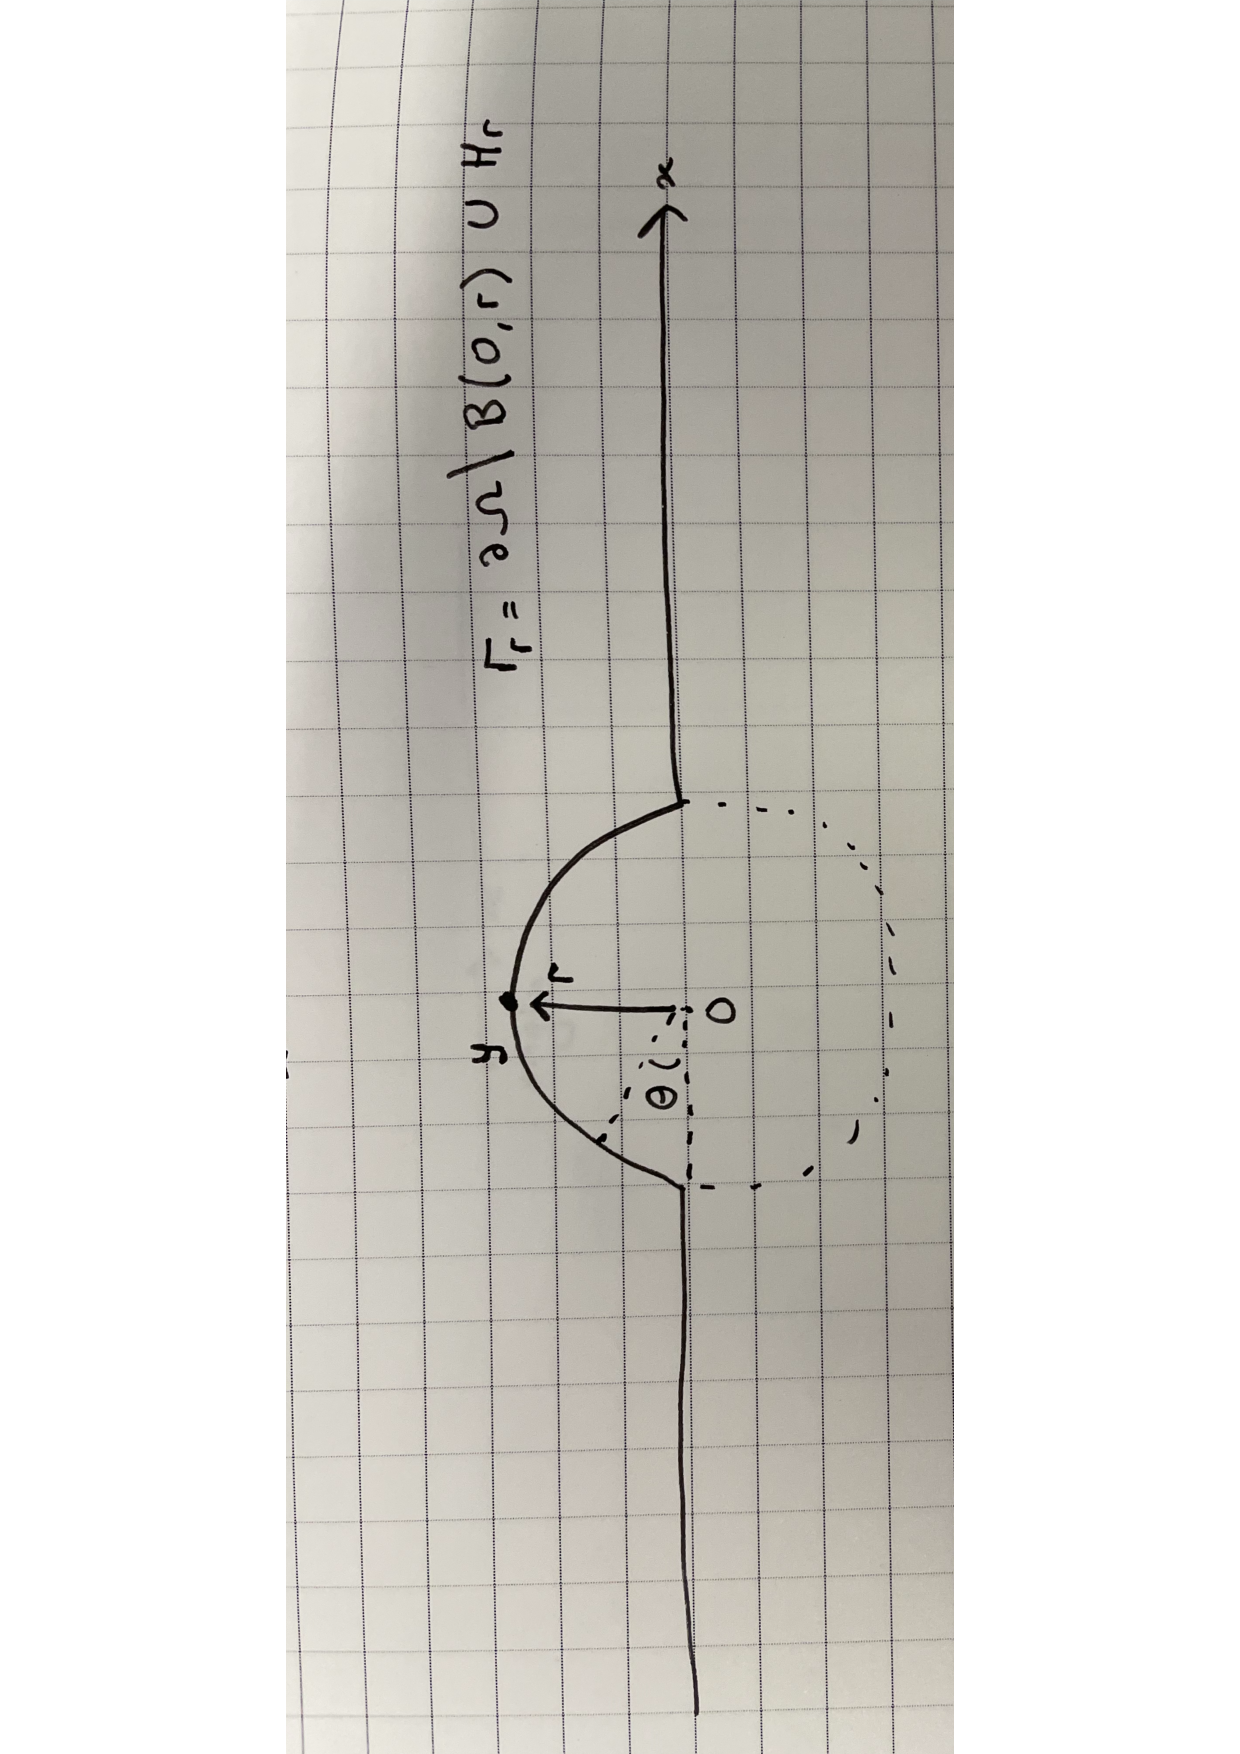
\includegraphics[width=0.6\textwidth, angle = -90]{fig1.pdf}
    \caption{Approaching a charged double layer of charge from outside the domain, right onto the origin.}
    \label{fig:laplace_double_jr}
\end{figure}

We create a half-sphere, $H_r$, with radius $r$ centered on the origin (and the singularity). For the Laplace kernel we get something like,

\begin{flalign}
    &\lim_{r \rightarrow 0} \left ( \frac{1}{2\pi} \int_{\Gamma_r} \frac{1}{|y|}ds \right ) \\
    &\lim_{r \rightarrow 0} \left (  \frac{1}{2\pi} \int_{H_r} \frac{1}{|y|}ds +  \frac{1}{2\pi} \int_{\partial \Omega \setminus B(0, r)} \frac{1}{|y|}ds \right )
\end{flalign}

Converting the integral over the half-sphere to polar coordinates,

\begin{flalign}
    \frac{1}{2\pi} \int_{0}^\pi \frac{r}{|r|} d\theta = \frac{1}{2}
\end{flalign}

We see that we get something of the form,

\begin{flalign}
    \label{eq:laplace_double_jr}
    v^+(x) = (\frac{1}{2} + \mathcal{D})[\psi(y)](x)
\end{flalign}

in the limit that $r \rightarrow 0$. The plus sign signifies that we approach the boundary from outside of the domain.

This is a bit of a hop skip and jump, but this is just to intuit where this could come from. This does in fact generalize to the Helmholtz case too, and to higher dimensions.

I'm fairly certain that this reasoning is invalid mathematically, as the the second integral above in the principal value sense (I still need to look up what this actually is).

\subsection{Helmholtz}

\subsection{Maxwell}


\printbibliography[heading=bibintoc]

\end{document}


